\documentclass[tikz,border=5pt]{standalone}
\usepackage{ctex}
\usepackage{pgfplots}
\pgfplotsset{compat=1.18}
\begin{document}
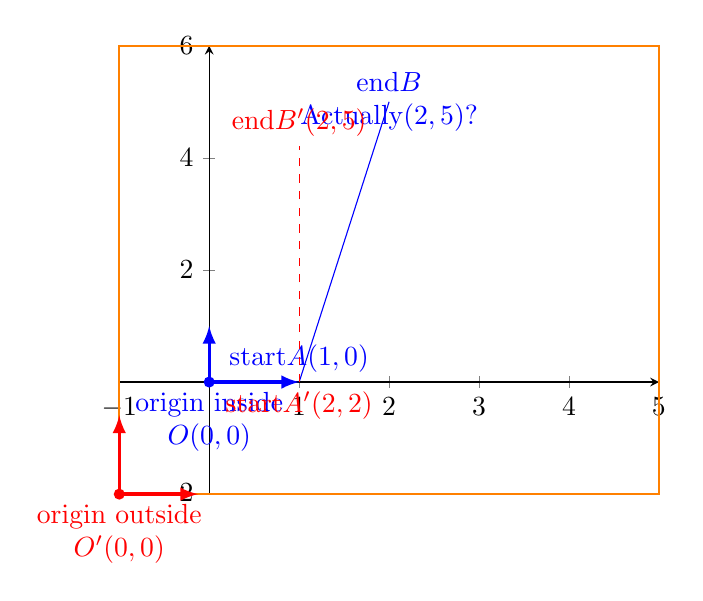
\begin{tikzpicture}
\begin{axis}[
        axis lines = middle,
        xmin = -1, xmax = 5,
        ymin = -2, ymax = 6,
        name = theAxis,
        % anchor=origin
    ]
    \coordinate (A) at (axis cs:1,0);
    \draw[blue] (A) node[above] {start$A(1,0)$} --++ (axis cs:0,3) node[align=center] {end$B$\\ Actually$(2,5)$?};
    \fill[blue] (0,0) circle[radius=2pt] node[below,align=center] {origin inside\\$O(0,0)$};
    \draw[-latex,blue,very thick] (0,0) -- (1,0);
    \draw[-latex,blue,very thick] (0,0) -- (0,1);
\end{axis}
    \draw [orange,thick] (theAxis.south west) rectangle (theAxis.north east);
    \draw[dashed,red] (A) node[below] {start$A'(2,2)$} --++ (0,3) node[above] {end$B'(2,5)$};
    \fill[red] (0,0) circle[radius=2pt] node[below,align=center] {origin outside\\$O'(0,0)$};
    \draw[-latex,red,very thick] (0,0) -- (1,0);
    \draw[-latex,red,very thick] (0,0) -- (0,1);
\end{tikzpicture}
\end{document}